\documentclass[tikz, border=10pt]{standalone}
\usetikzlibrary{calc, angles, quotes}
\begin{document}
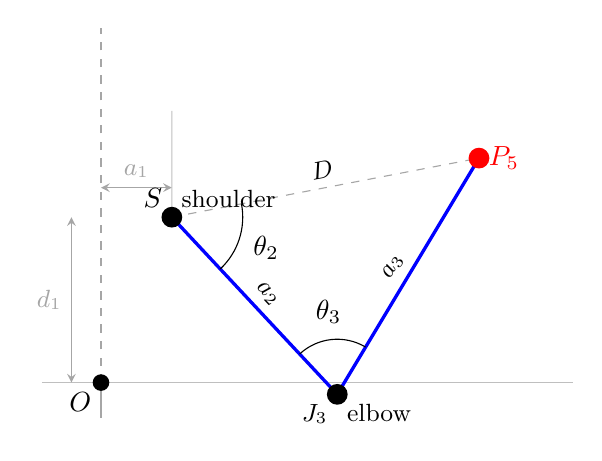
\begin{tikzpicture}[scale=1.5, >=stealth]

    % Parameters
    \def\aone{0.6}
    \def\done{1.4}
    \def\atwo{1.6}
    \def\athree{1.2}

    % Key points
    \coordinate (O) at (0,0);
    \coordinate (S) at (\aone, \done);
    \coordinate (P5) at (3.2, 1.9);
    \coordinate (J3) at ($ (S) + (1.4, -1.5) $);

    % Base axis
    \draw[gray!70, dashed] (O) -- (0, 3.0);
    \draw[gray!70] (O) -- (0, -0.3);

    % Horizontal reference
    \draw[gray!50, thin] (-0.5, 0) -- (4.0, 0);

    % Shoulder height d1
    \draw[<->, gray!70, thin] (-0.25, 0) -- (-0.25, \done);
    \node[left, gray!70, font=\small] at (-0.25, \done/2) {\(d_1\)};

    % Shoulder lateral offset a1
    \draw[<->, gray!70, thin] (0, \done+0.25) -- (\aone, \done+0.25);
    \node[above, gray!70, font=\small] at (\aone/2, \done+0.25) {\(a_1\)};

    % Upper arm (label above the line, sloped)
    \draw[blue, very thick] (S) -- (J3)
          node[midway, above, sloped, black, font=\small] {\(a_2\)};

    % Forearm (label above the line, sloped)
    \draw[blue, very thick] (J3) -- (P5)
          node[midway, above, sloped, black, font=\small] {\(a_3\)};

    % Distance D
    \draw[gray!70, dashed] (S) -- (P5)
          node[midway, above, sloped, black, font=\small] {\(D\)};

    % Vertical reference at the shoulder (for theta2)
    \draw[gray!50, thin] (S) -- (\aone, \done+0.9);

    % Angle theta2 at the shoulder
    \pic [draw, "\(\theta_2\)", angle radius=0.9cm, angle eccentricity=1.4]
         {angle = J3--S--P5};

    % Angle theta3 at the elbow
    \pic [draw, "\(\theta_3\)", angle radius=0.7cm, angle eccentricity=1.5]
         {angle = P5--J3--S};

    % Points and labels
    \fill (O) circle (2pt) node[below left] {\(O\)};
    \fill (S) circle (2.5pt) node[above left] {\(S\)};
    \fill (J3) circle (2.5pt) node[below left, font=\small] {\(J_3\)};
    \fill[red] (P5) circle (2.5pt) node[right] {\(P_5\)};

    % Optional: "shoulder" label, placed above S and away from the a1 arrow
    \node[above right, font=\small] at (S) {shoulder};

    % Optional: "elbow" label, placed below J3 and shifted right to avoid J3 overlap
    \node[below right, font=\small] at (J3) {elbow};

\end{tikzpicture}
\end{document}